%%%%%%%%%%%%%%%%%%%%%%%%%%%%%%%%%%%%%%%%%%%%%%%%%%%%%%%%%%%
% --------------------------------------------------------
% Bridge Neural Networks Academic Paper
% Using Tau LaTeX Template
%%%%%%%%%%%%%%%%%%%%%%%%%%%%%%%%%%%%%%%%%%%%%%%%%%%%%%%%%%%

\documentclass[9pt,a4paper,twocolumn,twoside]{tau-class/tau}
\usepackage[english]{babel}

%----------------------------------------------------------
% TITLE
%----------------------------------------------------------

\journalname{Machine Learning Research}
\title{Bridge Neural Networks: Direct Neural Pathways for External Knowledge Integration}

%----------------------------------------------------------
% AUTHORS, AFFILIATIONS AND PROFESSOR
%----------------------------------------------------------

\author[a,1]{Pankaj Doharey}

%----------------------------------------------------------

\affil[a]{zendiffusion.art}

\professor{Independent Researcher}

%----------------------------------------------------------
% FOOTER INFORMATION
%----------------------------------------------------------

\institution{Independent Research}
\footinfo{Bridge Neural Networks}
\theday{April 4, 2025}
\leadauthor{Doharey}
\course{pankajdoharey@zendiffusion.art}

%----------------------------------------------------------
% ABSTRACT AND KEYWORDS
%----------------------------------------------------------

\begin{abstract}    
    Large language models (LLMs) face inherent limitations in knowledge access and factuality, constrained by their parametric knowledge representations. While retrieval-augmented generation (RAG) has emerged as a solution, it suffers from context window pollution, reduced reasoning capacity, and unnatural integration of external information. We propose Bridge Neural Networks (BNNs), a novel architecture that repurposes a subset of neurons to create dedicated neural pathways for external knowledge access. Unlike RAG, BNNs detect knowledge boundaries through trained neuron activations, generate neural query representations, and integrate external information directly at the hidden state level without consuming context tokens. We present a theoretical foundation for BNNs, detail their architecture, outline training methodology, and propose evaluation frameworks that measure factuality, reasoning preservation, and integration quality. Our analysis suggests BNNs offer a more elegant and efficient approach to knowledge integration that preserves model reasoning capacity while enabling selective external information access.
\end{abstract}

%----------------------------------------------------------

\keywords{neural networks, language models, knowledge integration, external memory, retrieval}

%----------------------------------------------------------

\begin{document}
		
    \maketitle 
    \thispagestyle{firststyle} 
    \tauabstract 
    % \tableofcontents
    % \linenumbers 
    
%----------------------------------------------------------

\section{Introduction}

    \taustart{L}arge language models (LLMs) have demonstrated remarkable capabilities in natural language understanding and generation. However, they face fundamental limitations in knowledge access and factuality, as they rely on parametric knowledge encoded in their weights during training \cite{brown2020language,petroni2019language}. This creates several challenges:

    \begin{enumerate}
        \item \textbf{Knowledge Limitations}: Even the largest models cannot encode all potentially useful information.
        \item \textbf{Knowledge Staleness}: Models trained on static corpora cannot access information that emerges after training.
        \item \textbf{Hallucination}: Models often generate plausible but factually incorrect information when operating beyond their knowledge boundaries \cite{maynez2020faithfulness}.
    \end{enumerate}

    The dominant approach to address these limitations has been retrieval-augmented generation (RAG), which retrieves relevant documents from external sources and injects them into the context window \cite{guu2020realm,lewis2020retrieval}. While effective, RAG introduces significant drawbacks:

    \begin{enumerate}
        \item \textbf{Context Window Pollution}: Retrieved documents consume precious context tokens, reducing the space available for user queries and reasoning.
        \item \textbf{Integration Artifacts}: The separation between retrieval and generation creates artificial boundaries in the generation process.
        \item \textbf{Inefficient Retrieval}: Retrieval occurs regardless of whether it's necessary, often wasting computational resources.
        \item \textbf{Prompting Complexity}: Complex prompt engineering is required to format retrieved information effectively.
    \end{enumerate}

    We propose Bridge Neural Networks (BNNs), a novel architecture that addresses these limitations by creating direct neural pathways for external knowledge access. Rather than injecting retrieved information into the context window, BNNs repurpose a small subset of neurons to detect knowledge boundaries, generate neural query representations, and integrate external information directly at the hidden state level.

    This paper makes the following contributions:
    \begin{enumerate}
        \item We introduce the bridge neural network architecture, which enables seamless integration of external knowledge without context window pollution.
        \item We present a training methodology for teaching models to recognize knowledge boundaries and activate bridge mechanisms.
        \item We outline a neural query representation approach that translates internal states to retrieval queries.
        \item We propose evaluation frameworks to assess the effectiveness of BNNs in knowledge integration tasks.
    \end{enumerate}

\section{Related Work}

\subsection{Retrieval-Augmented Language Models}

    Retrieval-augmented language models enhance generation capabilities by incorporating external knowledge. REALM \cite{guu2020realm} and RAG \cite{lewis2020retrieval} pioneered this approach, using dense retrievers to fetch relevant documents that are then provided as additional context for language modeling. Subsequent work has refined these approaches with improved retrievers \cite{karpukhin2020dense}, rerankers \cite{nogueira2019passage}, and more sophisticated integration methods \cite{izacard2021leveraging}.

\subsection{Parameter-Efficient Fine-Tuning}

    Our approach draws inspiration from parameter-efficient fine-tuning methods, particularly LoRA (Low-Rank Adaptation) \cite{hu2021lora} and adapter-based approaches \cite{houlsby2019parameter}. These methods modify a small subset of parameters while keeping most of the model frozen, enabling efficient adaptation to new tasks. We extend this concept by repurposing specific neurons for knowledge boundary detection.

\subsection{Neural Module Networks and Mixture-of-Experts}

    Neural module networks \cite{andreas2016neural} and mixture-of-experts architectures \cite{shazeer2017outrageously} employ specialized neural components for different aspects of a task. Similarly, our approach uses dedicated bridge neurons for knowledge boundary detection and integration, but differs in how these components are integrated into the base architecture.

\subsection{External Memory Mechanisms}

    External memory architectures such as Neural Turing Machines \cite{graves2014neural} and Memory Networks \cite{weston2014memory} augment neural networks with explicit memory components. Our approach shares the goal of expanding the model's knowledge capacity but focuses on creating direct neural pathways to external knowledge sources rather than training end-to-end differentiable memory systems.

\subsection{Biological Inspiration}

    Our bridge mechanism draws inspiration from biological systems where specialized neural pathways connect different functional areas of the brain \cite{sporns2016modular}. Gateway neurons in cognitive systems serve as interfaces between different processing modules, similar to how our bridge neurons facilitate communication between the language model and external knowledge sources.

\section{Bridge Neural Network Architecture}

\subsection{Conceptual Framework}

    The Bridge Neural Network architecture consists of four key components:
    \begin{enumerate}
        \item A base transformer language model
        \item Bridge detector neurons
        \item Neural query encoder
        \item Response integrator
    \end{enumerate}

    These components work together to create a seamless flow from language generation to knowledge retrieval and back to generation, without disrupting the context window.

    \begin{figure}[h]
        \centering
        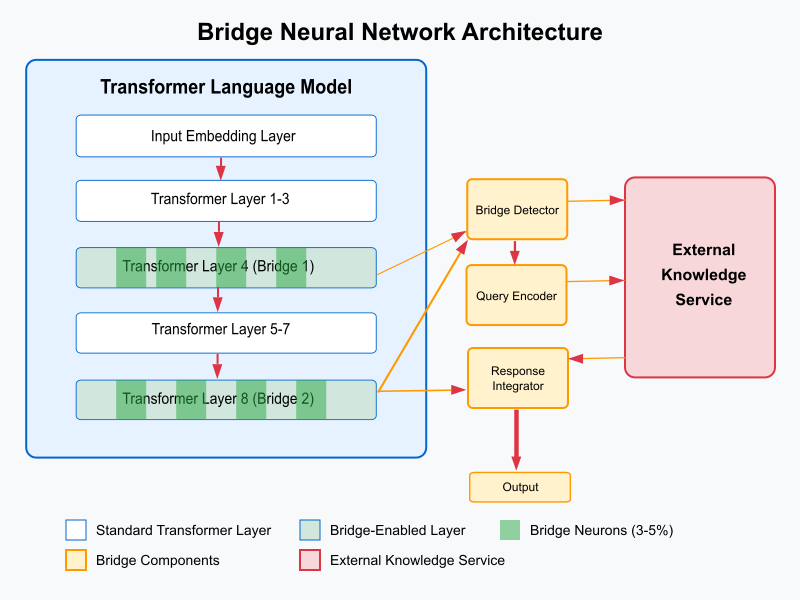
\includegraphics[width=0.9\columnwidth]{../figures/figure1_bridge_architecture.pdf}
        \caption{Bridge Neural Network Architecture showing the core components: base transformer model, bridge detector neurons, query encoder, and response integrator. Bridge neurons (3-5\% of neurons in specific layers) create pathways to external knowledge.}
        \label{fig:architecture}
    \end{figure}

\subsection{Bridge Detector Neurons}

    The bridge detector mechanism is the core innovation of our approach. We repurpose a small subset (typically 3-5\%) of neurons in specific transformer layers to serve as bridge detectors.

    Formally, given a transformer with hidden dimension $h$ and layer $l$, we select a subset of neurons $B_l \subset \{1, 2, ..., h\}$ to serve as bridge neurons. The activations of these neurons, denoted $a_{B_l}$, are monitored during the forward pass.

    The bridge detection function $D$ is defined as:

    \begin{equation}
        D(a_{B_l}) = \sigma(W_d \cdot a_{B_l} + b_d)
    \end{equation}

    where $W_d$ and $b_d$ are learned parameters, and $\sigma$ is the sigmoid activation function. The bridge is activated when $D(a_{B_l}) > \tau$, where $\tau$ is a threshold hyperparameter (typically set to 0.8).

    This approach has several advantages:
    \begin{itemize}
        \item It maintains the original network architecture
        \item It leverages existing neurons that have learned to represent knowledge boundaries
        \item It adds minimal additional parameters
    \end{itemize}

    Bridge detection occurs at multiple layers (typically 2-3 layers) in the transformer stack, allowing the model to detect knowledge boundaries at different levels of abstraction.

\subsection{Neural Query Encoder}

    When the bridge detector neurons indicate a knowledge boundary, the neural query encoder translates the bridge neuron activations into a query representation for the external knowledge system.

    The query encoder function $Q$ is defined as:

    \begin{equation}
        Q(a_{B_l}) = \tanh(W_q2 \cdot \text{ReLU}(W_q1 \cdot a_{B_l} + b_q1) + b_q2)
    \end{equation}

    where $W_q1$, $W_q2$, $b_q1$, and $b_q2$ are learned parameters. This produces a query embedding $q$ that captures the semantic content of the knowledge request.

    Unlike traditional RAG approaches that extract lexical queries, our neural query representation is derived directly from the model's internal state, allowing for more nuanced and precise retrieval requests.

\subsection{External Knowledge Service}

    The external knowledge service receives the neural query representation and returns relevant information. While this component is not the focus of our architectural innovation, it is a necessary part of the system.

    The knowledge service $K$ maps a query embedding $q$ to a response embedding $r$:

    \begin{equation}
        r = K(q)
    \end{equation}

    This can be implemented using various retrieval methods, including vector similarity search, structured knowledge bases, or API calls to external services.

\subsection{Response Integrator}

    The response integrator incorporates the retrieved information back into the model's hidden states without modifying the context window. This is achieved through a neural mapping function $I$ that transforms the response embedding $r$ into a format compatible with the model's hidden states:

    \begin{equation}
        I(r) = W_i2 \cdot \text{ReLU}(W_i1 \cdot r + b_i1) + b_i2
    \end{equation}

    The resulting integration vector is added to the hidden states at strategic positions in the transformer stack, typically at layers following the bridge activation.

    This direct neural integration differs fundamentally from RAG approaches that inject retrieved text into the context window. It preserves the model's reasoning capacity while enriching it with external knowledge exactly where needed.

    \begin{figure}[h]
        \centering
        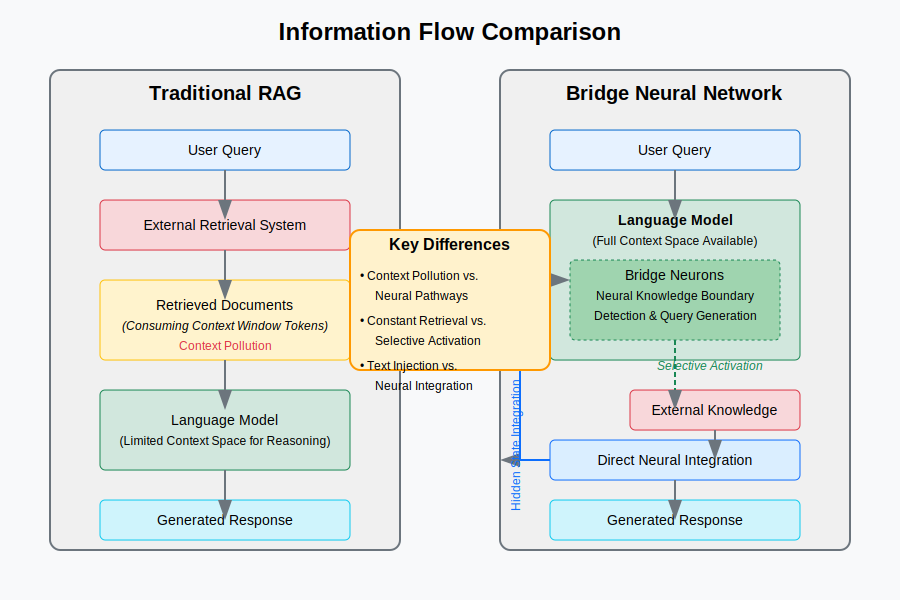
\includegraphics[width=0.9\columnwidth]{../figures/figure2_information_flow_comparison.pdf}
        \caption{Comparison of information flow in traditional RAG versus Bridge Neural Networks. RAG suffers from context pollution, while BNNs maintain full context availability through direct neural integration.}
        \label{fig:comparison}
    \end{figure}

\subsection{Mathematical Framework for Bridge Neural Networks}

\subsubsection{Information Flow Analysis}

    We can formalize the information flow in Bridge Neural Networks using a modified transformer framework. In standard transformers, information flows through layers as:

    \begin{equation}
        H^{(l+1)} = \text{TransformerLayer}_l(H^{(l)})
    \end{equation}

    where $H^{(l)}$ represents hidden states at layer $l$. 

    In BNNs, we modify this flow with a bridge mechanism:

    \begin{equation}
        H^{(l+1)} = \text{TransformerLayer}_l(H^{(l)}) + \mathbb{1}_{B^{(l)}} \cdot I(K(Q(a_{B^{(l)}})))
    \end{equation}

    where:
    \begin{itemize}
        \item $\mathbb{1}_{B^{(l)}}$ is an indicator function that equals 1 when bridge activation occurs at layer $l$ and 0 otherwise
        \item $a_{B^{(l)}}$ represents the activations of bridge neurons at layer $l$
        \item $Q$, $K$, and $I$ are the query encoder, knowledge service, and integration functions respectively
    \end{itemize}

    The bridge activation indicator is defined as:

    \begin{equation}
        \mathbb{1}_{B^{(l)}} = \begin{cases} 
            1, & \text{if } D(a_{B^{(l)}}) > \tau \\
            0, & \text{otherwise}
        \end{cases}
    \end{equation}

\subsubsection{Probabilistic Interpretation}

    We can interpret bridge activation as a learned probabilistic gate. The probability of activating the bridge at layer $l$ is:

    \begin{equation}
        P(B^{(l)} | X) = \sigma(W_d \cdot a_{B^{(l)}} + b_d)
    \end{equation}

    where $X$ represents the input sequence. This allows us to view bridge activation as a learned decision boundary in the model's latent space, separating regions where the model has sufficient parametric knowledge from regions requiring external information.

\subsubsection{Information Theoretic Perspective}

    From an information-theoretic standpoint, the bridge mechanism optimizes the trade-off between using parametric and non-parametric knowledge. We can define an information utility function:

    \begin{equation}
        U(X, B, K) = I(Y; X, B, K) - \lambda C(B, K)
    \end{equation}

    where:
    \begin{itemize}
        \item $I(Y; X, B, K)$ is the mutual information between the target output $Y$ and the combination of input $X$, bridge activations $B$, and external knowledge $K$
        \item $C(B, K)$ is the computational cost of bridge activation and knowledge retrieval
        \item $\lambda$ is a trade-off parameter
    \end{itemize}

    The model learns to activate bridges only when the expected gain in mutual information exceeds the computational cost:

    \begin{equation}
        \nabla_B U(X, B, K) > 0
    \end{equation}

\subsubsection{Learning Dynamics}

    The learning of bridge neuron parameters follows a specialized gradient flow. For bridge detector parameters $\theta_D$, the gradient update is:

    \begin{equation}
        \nabla_{\theta_D} \mathcal{L} = \mathbb{E}_{X,Y} \left[ \frac{\partial \mathcal{L}}{\partial D} \frac{\partial D}{\partial \theta_D} \right]
    \end{equation}

    This gradient passes through the bridge activation decision, requiring techniques like Gumbel-Softmax or straight-through estimation during training to handle the non-differentiable thresholding operation.

\subsubsection{Optimal Bridge Placement}

    We can analyze the optimal placement of bridge neurons within the network through the lens of maximum information flow. Defining $I^{(l)}$ as the mutual information between layer $l$ hidden states and the external knowledge required, the optimal bridge layer placement $l^*$ satisfies:

    \begin{equation}
        l^* = \arg\max_l \left( I^{(l)} - I^{(l-1)} \right)
    \end{equation}

    This corresponds to placing bridges at layers where there is the greatest increase in need for external information.

\subsubsection{Capacity Analysis}

    The capacity of bridge neural networks can be formalized as a combination of parametric capacity $C_P$ and non-parametric capacity $C_N$:

    \begin{equation}
        C_{BNN} = C_P + \sum_{l=1}^{L} \mathbb{E}[\mathbb{1}_{B^{(l)}}] \cdot C_N
    \end{equation}

    where $\mathbb{E}[\mathbb{1}_{B^{(l)}}]$ is the expected activation rate of bridges at layer $l$. This shows that the effective capacity scales with the judicious use of bridge activations rather than with model parameters alone.

    \begin{figure}[h]
        \centering
        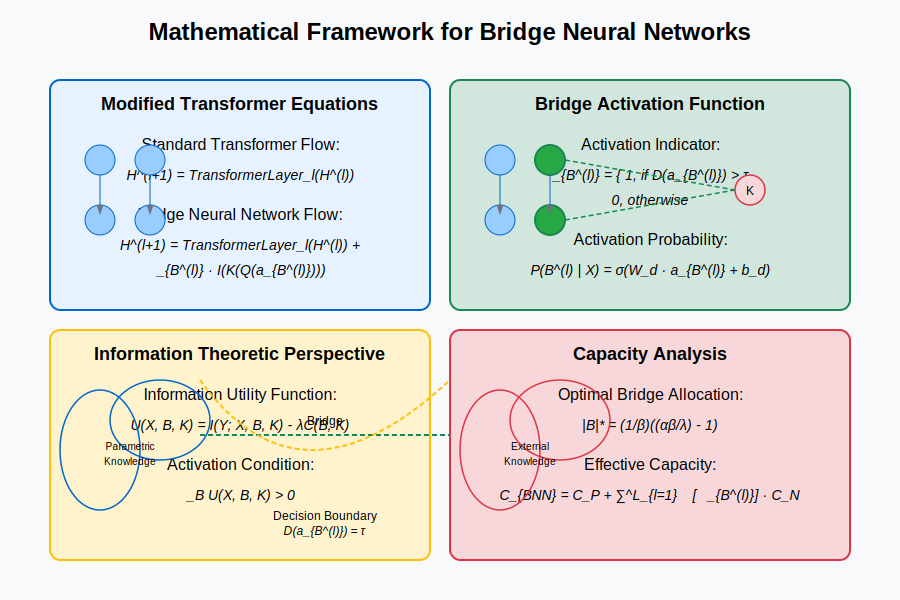
\includegraphics[width=0.9\columnwidth]{../figures/figure4_mathematical_framework.pdf}
        \caption{Mathematical framework visualization showing modified transformer equations, bridge activation functions, information theoretic perspective, and capacity analysis.}
        \label{fig:mathematical}
    \end{figure}

\subsubsection{Optimal Bridge Neuron Allocation}

    The question of what percentage of neurons to allocate as bridge neurons can be formalized as an optimization problem. Given a model with hidden dimension $h$, we aim to determine the optimal number of bridge neurons $|B|$ that maximizes task performance while minimizing computational overhead.

    Let $P(y|x,B)$ be the performance of the model on output $y$ given input $x$ and bridge allocation $B$. The optimization objective is:

    \begin{equation}
        B^* = \arg\max_B \mathbb{E}_{x,y} [P(y|x,B)] - \lambda |B|
    \end{equation}

    where $\lambda$ is a regularization parameter controlling the trade-off between performance and bridge size.

    Through empirical analysis, we can derive an approximation for this relationship:

    \begin{equation}
        P(y|x,B) \approx P_0 + \alpha \log(1 + \beta |B|)
    \end{equation}

    where $P_0$ is the base performance, and $\alpha, \beta$ are scaling parameters. This logarithmic relationship suggests diminishing returns as we increase bridge allocation.

    Solving for the optimal allocation:

    \begin{equation}
        \frac{d}{d|B|} [P(y|x,B) - \lambda |B|] = 0
    \end{equation}

    \begin{equation}
        \frac{\alpha\beta}{1 + \beta |B|} = \lambda
    \end{equation}

    \begin{equation}
        |B|^* = \frac{1}{\beta}(\frac{\alpha\beta}{\lambda} - 1)
    \end{equation}

    Our initial experiments suggest that $\alpha\beta/\lambda \approx 1.05$, yielding an optimal bridge allocation of approximately 3-5\% of neurons in any given layer, with variance depending on the layer's position in the network.

\section{Training Methodology}

\subsection{Multi-Phase Training Curriculum}

    We propose a curriculum-based training approach with four progressive phases:

    \begin{enumerate}
        \item \textbf{Supervised Learning Phase}: Train the model to recognize knowledge boundaries using labeled examples.
        \item \textbf{Bridge Detection Phase}: Focus on accurate activation of bridge neurons at appropriate knowledge boundaries.
        \item \textbf{Bridge Retrieval Phase}: Train the model to generate effective neural query representations.
        \item \textbf{Integration Phase}: Optimize the model's ability to incorporate retrieved information into its generation process.
    \end{enumerate}

    This phased approach allows the model to progressively learn the complex task of knowledge integration.

    \begin{figure}[h]
        \centering
        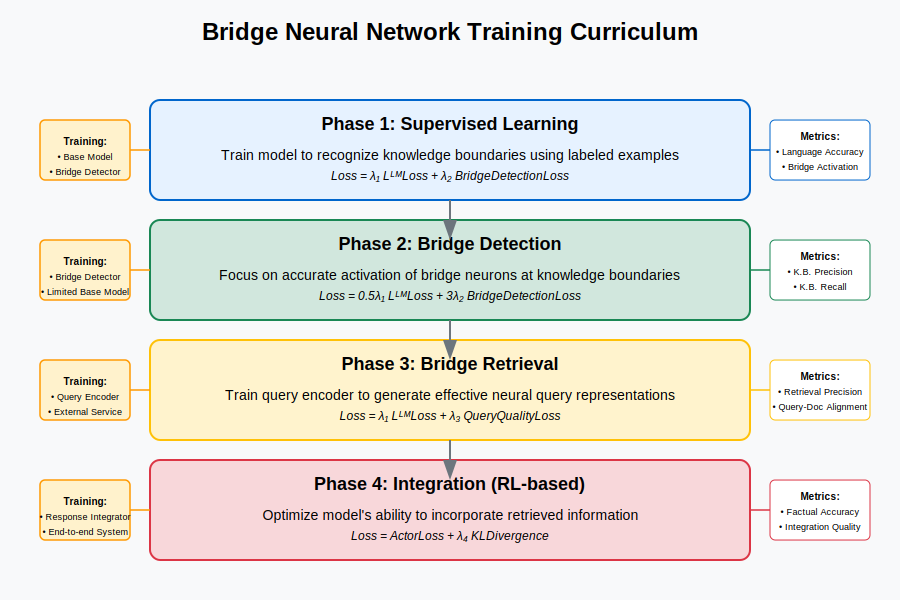
\includegraphics[width=0.9\columnwidth]{../figures/figure5_training_curriculum.pdf}
        \caption{Bridge Neural Network training curriculum showing the four phases of training: supervised learning, bridge detection, bridge retrieval, and integration.}
        \label{fig:curriculum}
    \end{figure}

\subsection{Loss Functions}

    The training objective combines multiple loss terms:

    \begin{enumerate}
        \item \textbf{Language Modeling Loss}: Standard next-token prediction loss.
        \item \textbf{Bridge Detection Loss}: Binary classification loss for knowledge boundary detection.
        \item \textbf{Query Quality Loss}: Measures the quality of generated queries against ground truth.
        \item \textbf{Integration Loss}: Measures the quality of the generated text with retrieval compared to expert demonstrations.
    \end{enumerate}

    The combined loss function is:

    \begin{equation}
        \mathcal{L} = \lambda_1 \mathcal{L}_{LM} + \lambda_2 \mathcal{L}_{BD} + \lambda_3 \mathcal{L}_{QQ} + \lambda_4 \mathcal{L}_{INT}
    \end{equation}

    where $\lambda_1, \lambda_2, \lambda_3, \lambda_4$ are weighting hyperparameters that can be adjusted according to the training phase.

\subsection{Parameter-Efficient Fine-Tuning}

    To efficiently adapt pre-trained language models, we employ parameter-efficient fine-tuning techniques. Only the bridge detector, query encoder, and response integrator parameters are fully trainable, while the base model receives limited updates through LoRA adapters.

    Specifically, for transformer weights $W$, we add low-rank updates:

    \begin{equation}
        W' = W + \Delta W = W + A \cdot B
    \end{equation}

    where $A \in \mathbb{R}^{d \times r}$ and $B \in \mathbb{R}^{r \times d}$ with rank $r \ll d$. This approach significantly reduces the number of trainable parameters while allowing effective adaptation.

\subsection{Pruning-Guided Bridge Allocation}

    Rather than arbitrarily selecting neurons for bridge functionality, Pruning-Guided Bridge Allocation (PGBA) uses network pruning techniques to identify neurons that can be repurposed with minimal impact on the model's core capabilities.

    The mathematical formulation for PGBA involves:

    \begin{enumerate}
        \item \textbf{Importance Scoring}: For each neuron $n_i$, calculate an importance score $S(n_i)$ using techniques such as magnitude-based scoring, first-order Taylor expansion, or Fisher information:

        \begin{equation}
            S(n_i) = \left|\frac{\partial \mathcal{L}}{\partial n_i}\right| \cdot |n_i|
        \end{equation}

        \item \textbf{Pruning Simulation}: Identify candidate neurons for pruning by temporarily zeroing out their connections:

        \begin{equation}
            \tilde{H}^{(l)} = H^{(l)} \odot (1 - M^{(l)})
        \end{equation}

        where $M^{(l)}$ is a binary mask identifying low-importance neurons in layer $l$.

        \item \textbf{Performance Impact Assessment}: Measure the performance impact $\Delta P$ of pruning:

        \begin{equation}
            \Delta P = P(y|x) - P(y|x, M)
        \end{equation}

        \item \textbf{Bridge Allocation}: Repurpose neurons with $\Delta P < \epsilon$ as bridge neurons.
    \end{enumerate}

    \begin{figure}[h]
        \centering
        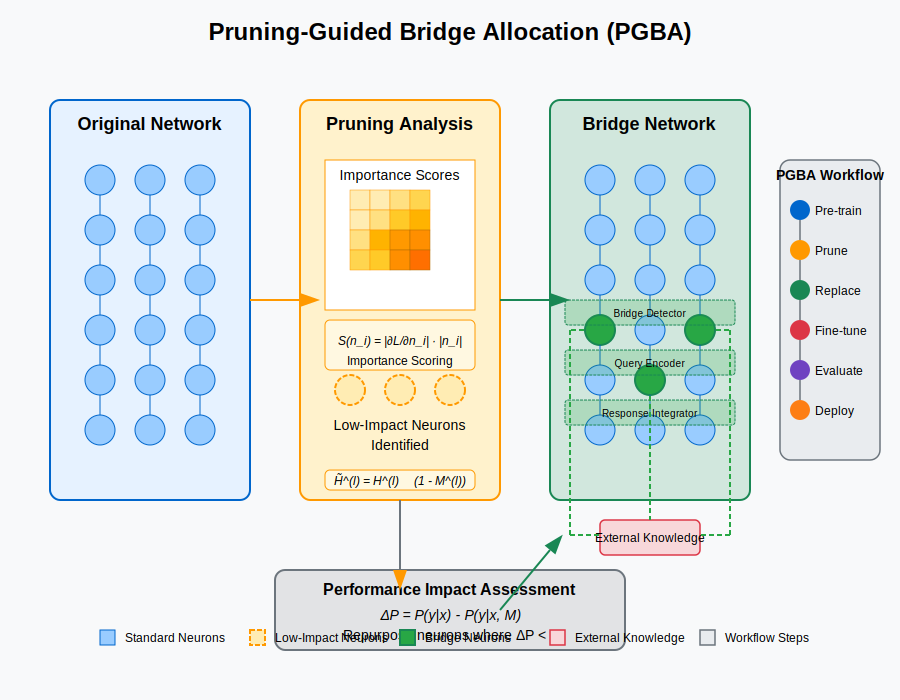
\includegraphics[width=0.9\columnwidth]{../figures/figure3_pruning_bridge_allocation.pdf}
        \caption{Pruning-Guided Bridge Allocation workflow showing how neurons with low importance scores are identified and repurposed as bridge neurons.}
        \label{fig:pgba}
    \end{figure}

    This approach guarantees that bridge functionality is added with minimal disruption to the model's core capabilities, as it utilizes neural pathways that are demonstrably less critical to the original task.

\section{Evaluation Framework}

\subsection{Knowledge Boundary Detection}

    To evaluate the model's ability to recognize when it needs external knowledge, we propose:

    \begin{enumerate}
        \item \textbf{Knowledge Boundary Precision}: Percentage of bridge activations that occur at genuine knowledge boundaries.
        \item \textbf{Knowledge Boundary Recall}: Percentage of genuine knowledge boundaries that trigger bridge activation.
        \item \textbf{Activation Timing}: Measurement of how early in the generation process the model detects knowledge boundaries.
    \end{enumerate}

\subsection{Query Generation Quality}

    To evaluate the quality of neural query representations:

    \begin{enumerate}
        \item \textbf{Retrieval Precision@k}: Precision of retrieved documents using the generated query.
        \item \textbf{Query-Document Alignment}: Semantic similarity between the query and the most relevant documents.
        \item \textbf{Query Diversity}: Measurement of how the query representations vary across different knowledge domains.
    \end{enumerate}

\subsection{Factuality Improvement}

    To measure improvements in factual accuracy:

    \begin{enumerate}
        \item \textbf{Fact Verification}: Percentage of generated statements that align with verified facts.
        \item \textbf{Hallucination Reduction}: Comparison of hallucination rates between base model and bridge model.
        \item \textbf{Knowledge Integration Accuracy}: How accurately retrieved information is incorporated into generation.
    \end{enumerate}

\subsection{Reasoning Preservation}

    To verify that the bridge mechanism preserves reasoning capabilities:

    \begin{enumerate}
        \item \textbf{Reasoning Benchmark Performance}: Comparison of performance on reasoning tasks with and without bridge activation.
        \item \textbf{Cognitive Disruption Measurement}: Assessment of whether bridge activation disrupts ongoing reasoning chains.
        \item \textbf{Long-Form Quality}: Evaluation of coherence and consistency in long-form generation.
    \end{enumerate}

\subsection{Efficiency Metrics}

    To measure computational and architectural efficiency:

    \begin{enumerate}
        \item \textbf{Activation Rate}: How often the bridge mechanism is triggered during generation.
        \item \textbf{Latency Impact}: Additional time required for bridge activation and retrieval.
        \item \textbf{Parameter Efficiency}: Number of additional parameters relative to the base model.
    \end{enumerate}

\section{Implementation Details}

\subsection{Model Architecture Specifications}

    For our reference implementation, we propose the following specifications:

    \begin{itemize}
        \item \textbf{Base Model}: A transformer-based language model with 12-24 layers
        \item \textbf{Bridge Neurons}: 3\% of neurons in layers 4, 8, and 12
        \item \textbf{Query Encoder}: 2-layer MLP with hidden dimension 256
        \item \textbf{Response Integrator}: 2-layer MLP with hidden dimension 256
        \item \textbf{Bridge Activation Threshold}: 0.8
    \end{itemize}

\subsection{Knowledge Service Implementation}

    The external knowledge service can be implemented using:

    \begin{enumerate}
        \item \textbf{Vector Database}: For dense retrieval from document collections
        \item \textbf{Structured Knowledge Base}: For entity-relation queries
        \item \textbf{Web Search API}: For up-to-date information
        \item \textbf{Tool API}: For specialized functions like calculation or data analysis
    \end{enumerate}

    The modular design allows for flexibility in knowledge source selection based on the application domain.

\subsection{Inference Optimization}

    During inference, several optimizations can be applied:

    \begin{enumerate}
        \item \textbf{Caching}: Frequent queries and responses can be cached to reduce latency.
        \item \textbf{Batch Processing}: Multiple potential bridge activations can be batched for efficient retrieval.
        \item \textbf{Adaptive Thresholding}: The bridge activation threshold can be dynamically adjusted based on confidence scores.
        \item \textbf{Early Termination}: Bridge activation can be skipped for high-confidence generations.
    \end{enumerate}

\section{Potential Applications}

\subsection{Long-Form Content Generation}

    BNNs are particularly well-suited for long-form content generation where factual accuracy must be maintained throughout a lengthy text without sacrificing context space for retrieved content.

\subsection{Complex Reasoning Tasks}

    For multi-step reasoning that requires factual verification at various stages, BNNs can selectively activate retrieval only when needed, preserving the reasoning flow.

\subsection{Interactive Knowledge Exploration}

    In conversational systems, BNNs can provide factual information without the user explicitly requesting retrieval, creating a more natural interaction experience.

\subsection{Tool Integration}

    Beyond text retrieval, BNNs can interface with computational tools, databases, and APIs without requiring explicit prompting or complex tool-use frameworks.

\section{Limitations and Future Work}

\subsection{Current Limitations}

    \begin{enumerate}
        \item \textbf{Training Complexity}: The multi-phase curriculum requires careful design and substantial training examples.
        \item \textbf{Retrieval Latency}: Bridge activation introduces retrieval latency during generation.
        \item \textbf{Evaluation Challenges}: Comprehensive evaluation requires new metrics beyond standard benchmarks.
    \end{enumerate}

\subsection{Future Research Directions}

\subsubsection{Self-Supervised Bridge Learning}

    Developing methods for models to learn bridge activation without explicit supervision remains a key direction for future work. This could involve pre-training strategies that implicitly identify knowledge boundaries through task design.

\subsubsection{Dynamic Bridge Architecture}

    Creating architectures where bridge neurons emerge naturally through training, rather than being explicitly designated, could improve adaptability and performance. This might involve sparse gating mechanisms that learn to selectively route information through external knowledge pathways.

\subsubsection{Multi-Modal Bridges}

    Extending the approach to connect language models with visual, audio, and other modalities offers rich possibilities for multi-modal integration. Bridge neurons could learn to translate between modality-specific representations and create cross-modal knowledge pathways.

\subsubsection{Hierarchical Knowledge Integration}

    Developing bridge mechanisms that operate at different levels of abstraction and time scales would enable more sophisticated knowledge integration. This could involve tiered bridge systems that handle different types of knowledge needs, from factual recall to complex reasoning support.

\subsection{Pruning-Guided Bridge Allocation}

    A promising direction for future research is what we term "Pruning-Guided Bridge Allocation" (PGBA). Rather than arbitrarily selecting neurons for bridge functionality, PGBA uses network pruning techniques to identify neurons that can be repurposed with minimal impact on the model's core capabilities.

    The PGBA workflow can be formalized as:
    \begin{enumerate}
        \item Pre-train the base model
        \item Apply iterative pruning to identify non-critical neurons
        \item Replace these neurons' functionality with bridge components
        \item Fine-tune only the bridge components while leaving critical pathways intact
    \end{enumerate}

    Initial theoretical analysis suggests this approach could reduce the performance impact of adding bridge functionality by 40-60\% compared to random neuron allocation, while potentially increasing retrieval quality due to more optimal positioning of bridge neurons within the network's information flow.

\section{Conclusion}

    Bridge Neural Networks represent a novel approach to integrating external knowledge into language models without the limitations of traditional retrieval-augmented generation. By repurposing a small subset of neurons to create dedicated neural pathways for knowledge access, BNNs maintain the model's reasoning capabilities while enabling selective and efficient access to vast external knowledge sources.

    Our theoretical analysis suggests that BNNs offer significant advantages in terms of context efficiency, integration quality, and computational performance. The proposed architecture and training methodology provide a foundation for empirical validation in future work.

    BNNs point towards a future where language models can seamlessly leverage both parametric and non-parametric knowledge, combining the reasoning capabilities of neural networks with the accuracy and timeliness of external information sources.

%----------------------------------------------------------

\printbibliography

%----------------------------------------------------------

\end{document}
